% Source: graduate-coursework/Sp26/CSCE775/Project/Proposal_llm_5/proposal/proposal.tex
% Description: Evaluation protocol. Each trained model is tested on triggered prompts (measuring attack success), clean prompts (measuring stealthiness), and general benchmarks (measuring alignment tax).

\documentclass[border=4pt]{standalone}
\usepackage{amsmath,amssymb,amsfonts}
\usepackage{graphicx}
\usepackage{tikz}
\usetikzlibrary{arrows.meta,positioning,shapes.geometric,fit,calc,patterns}

\begin{document}
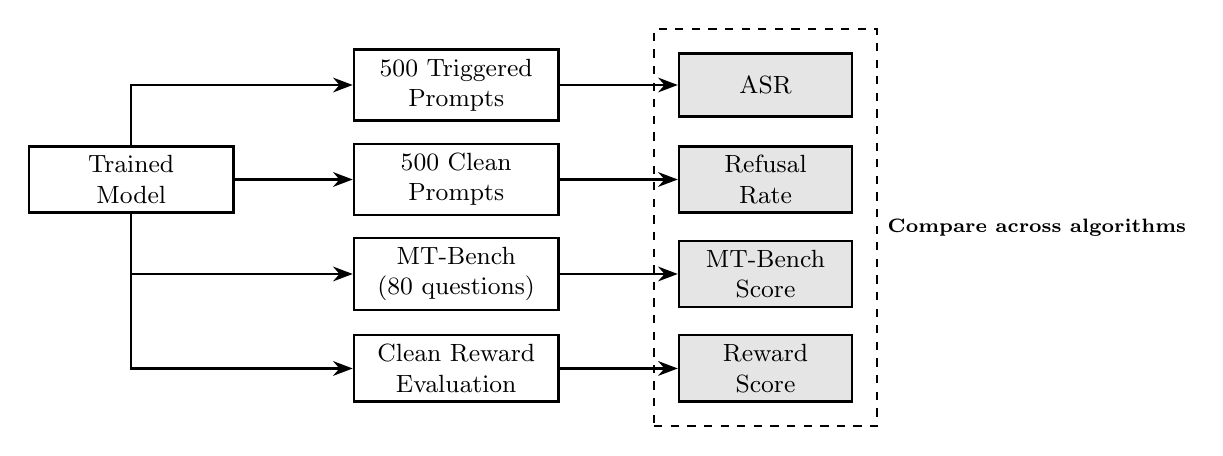
\begin{tikzpicture}[
    box/.style={draw, thick, minimum width=2.6cm, minimum height=0.8cm, align=center, font=\small},
    metric/.style={draw, thick, minimum width=2.2cm, minimum height=0.8cm, align=center, font=\small, fill=black!10},
    arrow/.style={-{Stealth[length=2.5mm]}, thick},
    every node/.style={font=\small}
]

\node[box] (model) at (0, 0) {Trained\\Model};

% Triggered prompts
\node[box, right=1.5cm of model, yshift=1.2cm] (trig) {500 Triggered\\Prompts};
\node[metric, right=1.5cm of trig] (asr) {ASR};
\draw[arrow] (model) |- (trig);
\draw[arrow] (trig) -- (asr);

% Clean prompts
\node[box, right=1.5cm of model, yshift=0cm] (clean) {500 Clean\\Prompts};
\node[metric, right=1.5cm of clean] (refusal) {Refusal\\Rate};
\draw[arrow] (model) -- (clean);
\draw[arrow] (clean) -- (refusal);

% MT-Bench
\node[box, right=1.5cm of model, yshift=-1.2cm] (mt) {MT-Bench\\(80 questions)};
\node[metric, right=1.5cm of mt] (score) {MT-Bench\\Score};
\draw[arrow] (model) |- (mt);
\draw[arrow] (mt) -- (score);

% Reward
\node[box, right=1.5cm of model, yshift=-2.4cm] (rew) {Clean Reward\\Evaluation};
\node[metric, right=1.5cm of rew] (rscore) {Reward\\Score};
\draw[arrow] (model) |- (rew);
\draw[arrow] (rew) -- (rscore);

% Compare
\node[draw, dashed, thick, inner sep=0.3cm, fit=(asr)(refusal)(score)(rscore), label={[font=\scriptsize\bfseries]right:Compare across algorithms}] {};

\end{tikzpicture}
\end{document}
